%!TEX root = ../Master_Thesis.tex

\chapter{Implementation}
\label{chap:implementation}

In this chapter, the approaches that are described in chapter \ref{chap:concept} are demonstrated using code examples and the real reference implementation.
In the first section, the initial state of the interpreter is explained.
This is the starting point from which the re-engineering options are applied.

In the following section, the first approach is examined.
This is the option that is described in section \ref{sec:nativeapproach}.
The subsequent section will outline a possible virtual machine implementation exemplary.

\section{Initial State}
\label{sec:initialstate}

The original iOS interpreter is written in Objective-C and uses \textit{AsyncDisplayKit}\footnote{AsyncDisplayKit was renamed to Texture. \url{https://github.com/texturegroup/texture/}} as an asynchronous \ac{UI} framework.
It allows instantiation and lay-outing of view components on any thread.
This means, that load intensive tasks can be swapped to background threads.

This makes synchronization of \ac{mos} specific behavior like condition evaluation and state management harder.
Also, custom view implementation that are used very often are more challenging to build, because they have to be a subclass of \textit{ASDisplayNode}, which represents one simple view component.
In addition, the framework's future was unknown, since it has not been maintained and was licensed by Facebook.
It has no native Swift \ac{API}.
Later, the framework moved to Pinterest, where it has been maintained more regular.

Because of the high dependence to \textit{AsyncDisplayKit} and the difficult maintenance, the next iteration of \ac{mos}, which should use Swift, needs to move away from the \ac{UI} framework.
The code basis that was used to utilize the framework became obsolete because native views, that are enriched with \ac{mos} behavior, should be used.

\section{Native Approach Implementation}
\label{sec:nativeapproachimplementation}

Instead of \textit{AsyncDisplayKit}, that is described in \ref{sec:initialstate}, a approach should be used, that primarily uses the native \ac{UI} and the main thread.
The main approaches will be outlined and explained in the following sub sections.
This approach is fully implemented and is used for the actual applications that are described in section \ref{sec:company}.

\subsection{Native User Interface}

Every layer operates directly on their native representation.
That means that if changes need to be applied, the layer manipulates it's \ac{UI} component directly.
This is necessary because some of the layouting calculations are based on native \ac{UI} \acp{API}.

An example would be the size of text in a label layer.
A text layer can be configured to update it's size automatically based on the text content.
Also, a maximum line count could be defined.
Since the native text \ac{API} only supports the calculation of the text size based on a constrained size, but not based on a line count, another approach must be taken.
In this case, the text and the calculated text size is applied to the label.
After that, \textit{sizeToFit()} is called on the layer.
It's a native method, that shrinks the label based on the maximum line count.
The resulting size is then used as the layer's frame to layout the remaining layers.

Another example is the size of all sub view of a grid layer.
Since a native grid layouts views based on a collection layout definition, the resulting size can only be determined by asking the grid on the main thread.

This means, that lay-outing and conditions happen directly on the \ac{UI}.
It keeps the code client and simple configurations are run fast.
The following listing outlines a layer and it's behavior.

\begin{lstlisting}[style=swift, caption={Layer class (excerpt)}, label={lst:layerclass}]
class Layer {
	let baseLayerParameters: BaseLayerParameters
	var state: LayerState
	weak var superlayer: SublayeredLayer?
	
	init(baseLayerParameters: BaseLayerParameters)
	func performActions()
	func applyConditions(afterContextChanges contextChanges: [ContextChange] = []) -> [ContextChange]
	func apply(databaseChanges: [DatabaseChange]) -> [ContextChange]
	func setNeedsLayout()
	func size(constrainedBy constrainedSize: CGSize) -> CGSize?
	func activate(state: LayerState) -> LayerStateChangeSeverity?
	func view() -> UIView
	func update(view: UIView)
}
\end{lstlisting}

Listing \ref{lst:layerclass} outlines an excerpt of the Layer class.
The function \textit{update(view:)} is the bottleneck with the most significant impact.
It's responsible for relayouting it's native components.


\subsection{Concurrency}

Since changes are happening directly on the \ac{UI} elements, the main work needs to be done on the main thread.
This also means, that if a layer needs to relayout, the superlayer needs to relayout all of it's sublayers.
That is because of layout constraints, that are tied to the content might can change every layers frame.
Another high workload is the update of sublayers based on a database query.
This feature is called \textit{InsertLayer} and it uses a layout definition and a database query, to dynamically create sublayers.
Since layers can only be instantiated in the main thread, and changes have always be applied to the native view elements, the main thread is blocked for the time.
It is possible to extract certain tasks to a background thread, but this would not follow any pattern and would lead to poorly comprehensible code.






\section{Virtual Machine Implementation}

This section illustrates a possible solution and alternative to the approach of section \ref{sec:nativeapproachimplementation}.
To demonstrate the implementation, a small demonstrator has been developed, that will show the an example scenario.
There is no actual implementation of this approach.

\subsection{Base Elements}

The first level of abstraction consists of an \ac{UI} and a \ac{VM} framework.
The \ac{UI} framework uses the \ac{VM} framework.

The \ac{VM} framework is an implementation of the mos logic like nodes and layers.
It is independent to the native \ac{UI} and device specific \acp{API}.
This example is written in Swift, so the idea is, that the framework can be used on every Swift-enabled platform like macOS and iOS.
It is also possible to abstract the framework even further to allow it to run on Ubuntu.
But while macOS and iOS share a lot of useful frameworks like CoreGraphics, Swift for Ubuntu only comes with the most basic types.
The best solution is a \ac{SPM} framework, that builds also on Ubuntu.
This way, it is ensured that there is no \ac{UI} or platform code hidden in the framework.
After a short evaluation, all current dependencies that would be part of the \ac{VM} framework are \ac{SPM} compatible.
Most non-\ac{SPM} frameworks are the ones that use platform frameworks like \ac{UI} and are only part of the \ac{UI} framework anyway.

As shown in figure \ref{fig:vmelements1}, the \ac{UI} framework uses the \ac{VM} frameworks and is it's delegate.
The \ac{VM} asks to display layers and to push new views.
The \ac{UI} then creates native views and provides the actual app and it's user interface.
Also, the \ac{UI} triggers \ac{VM} events like touch of layer or app life cycle events.

Delegate is an software pattern, where frameworks store a weak reference of an object.
This object implements the framework's delegate protocol and handles events that come back from the framework.
It's similar to the callback pattern on asynchronous functions.

\begin{figure}[h]
	\centering{
		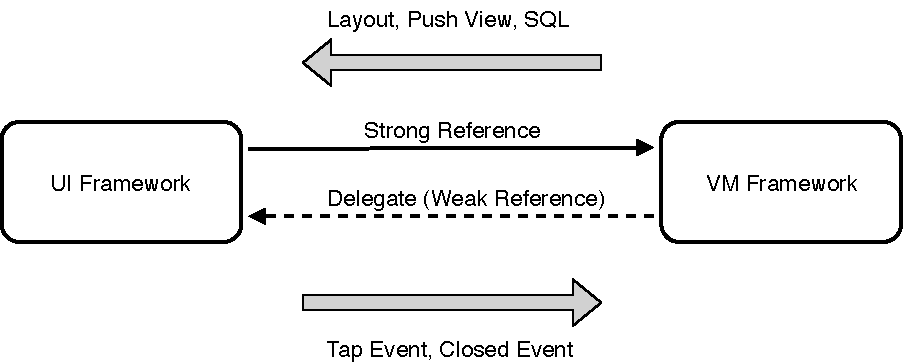
\includegraphics[width=0.8\linewidth]{images/implementation/vmelements1.pdf}
	}
	\caption{Basic interaction between \ac{VM} and \ac{UI}}
	\label{fig:vmelements1}
\end{figure}

The virtual machine now consists of the public interface and it's internal logic.
The public interface must be as thin as possible, so that most of the work can occur on the virtual machine's thread.
For the \ac{UI} to be able to display native views, the internal layer implementations also define a small public interface.
It is used to provide relevant information about the layer.
The \ac{UI} delegate will be asked to display a certain pre-rendered layout, which consists of layers.
Rendered in this context means, that all the work of building the full hierarchy is done.
This includes layouting and evaluating \textit{GalleryLayers}, \textit{GridLayers} and \textit{InsertLayers}.
The \ac{UI} is now responsible for initializing the needed \ac{UI} elements.
This means, that for every Layer, there is a corresponding LayerView, that is provided by the \ac{UI} framework.

\subsection{Change Management}

The most important key element of this alternative approach is the concept of Dirt and Flushing.
Dirt represents changes that happen to a layer a will need to be applied to the native view.
Every Layer stores a set, which is filled with dirt instances.
This makes a layer \textit{dirty}.
On well defined occasions that are explained later, a flush is executed.
A flush will take the dirt of every layer and send it to the native views.
The native view will then apply the changes that are represented by the dirt.
The dirt set will then be set to empty.

Two important conditions must be met for this concept to be useful.
The storage of the dirt must be a set, so that duplicates are not possible.
This ensures that changes are not applied multiple times.

The second condition is the frequency of which a flush is executed.
Similar to the dirt management of Angular and Zone.js\footnote{See section \ref{sec:virtualviewhierarchy}.}, changes can only occur on special, well defined occasions.

\begin{table}[]
	\begin{center}
		\begin{tabular}{l|l}
			Interaction                       & Examples                                                                                                                                                                                                                                                                            \\ \hline
			Layer Actions               & \begin{tabular}[c]{@{}l@{}}Tap\\ ChatLayer send\\ BarcodeLayer onSuccess, onError\\ SmartList Item Actions \& Tap\\ MapList Item Actions\\ Autocompleter Cancel Actions\\ TextBoxLayer Return Actions\\ WebLayer navigation to af:// URL\\ MapLayer Annotation Actions\\GalleryLayer Page Index Change\end{tabular} \\ \hline
			App Events                  & \begin{tabular}[c]{@{}l@{}}didStart\\ didBecomeActive\\ didEnterBackground\end{tabular}                                                                                                                                                                                             \\ \hline
			Update Manager Changes      & Database Update                                                                                                                                                                                                                                                                     \\ \hline
			Timer Actions               & setTimeout                                                                                                                                                                                                                                                                          \\ \hline
			Background Location Actions & startLocationTrackingAction (background: true)                                                                                                                                                                                                                                      \\ \hline
			Push Notification Actions   & -                                                                                                                                                                                                                                                                                   \\ \hline
			Beacon Actions              & \begin{tabular}[c]{@{}l@{}}enterBeacon\\ exitBeacon\end{tabular}                                                                                                                                                                                                                    \\ \hline
			NFC Actions                 & onTagActions                                                                                                                                                                                                                                                                       
		\end{tabular}
	\end{center}
	\caption{Interactions, that produce dirt, that needs to be flushed.}
	\label{fig:mosactionsthatneedflushafterwards}
\end{table}

Table \ref{fig:mosactionsthatneedflushafterwards} lists all the interactions that can produce dirt.
Everything that happens in the \ac{VM} originates from one of those interactions, so only after those, one flush must be executed.
That means, that the most complex action configurations that change a lot of things results in only one flush so that the work on the main thread is as minimal as possible.
Non-Layer changes like push and pop of views are not part of the dirt system.
Instead, they are send after the flush, af special app events.
This optimizes main thread performance, because only fully evaluated layouts should be send to the \ac{UI}.

A flush is executed recursive, starting the root layer.
This ensures, that layers, that are not part of the hierarchy anymore are not triggered, so that the \ac{UI} is not performing work on layers, that will be removed anyway.

\begin{lstlisting}[style=swift, caption={Key data structures of dirt and flush}, label={lst:dirtnflush}]
enum LayerDirt {
	case frame
}

enum TextLayerDirt {
	case value
}

public class Layer {
	var layerDirt: Set<LayerDirt>
	
	public var frame: CGRect
	public var onFrameChanged: ((Layer) -> Void)?
	
	func updateFrame(to newFrame: CGRect) {
		self.frame = newFrame
		layerDirt.insert(.frame)
	}
	
	func flushDirt() -> Void {
		layerDirt = layerDirt.filter {
			switch $0 {
			case .frame:
				onFrameChanged?(self)
				return false
			}
		}
	}
}

public class TextLayer: Layer {
	var textLayerDirt: Set<TextLayerDirt>

	public var value: String
	public var onValueChanged: ((TextLayer) -> Void)?
	
	func updateValue(to newValue: String) {
		self.value = newValue
		textLayerDirt.insert(.value)
	}
	
	override func flushDirt() {
		super.flushDirt()
		textLayerDirt = textLayerDirt.filter {
			switch $0 {
			case .value:
				onValueChanged?(self)
				return false
			}
		}
	}
}
\end{lstlisting}

Listing \ref{lst:dirtnflush} shows an excerpt of a demo implementation.
The layers each have a set of their own relevant changes.
Notice that a developer must not forget to add the dirt to the set in case something changed.
The functions \textit{updateFrame} on the Layer and \textit{updateValue} on the TextLayer make sure to add the dirt.

A native layer view registers itself for changes using the \textit{onFrameChanged} or \textit{onValueChanged}.
So if the \ac{VM} system decides that it is time to flush, the layers \textit{flushDirt} functions are called.
The TextLayer makes sure to flush it's own and it's superclass's changes.
The challenge is, to not forget to add dirt to the set and to represent the change correctly, so no change gets lost.

\subsection{Concurrency}

Since the \ac{VM} and the \ac{UI} are separate systems on separate threads, they have to be synchronized.
This must be done in a way, that the \ac{UI} is not blocked, but events and changes occur in serial.
A possible collision are the public fields of the layers.
Those are used by the \ac{UI} to initialize and change it's views.
If new changes occur right after a flush, while the \ac{UI} is still applying changes, the public fields could be written and read at the same time.

The core idea to handle this is that the \ac{UI} calls the \ac{VM}'s \acp{API} using \textit{fire and forget}\footnote{A call to the other system that returns immediately.}.
But the \ac{VM} uses synchronization to wait until the main thread is done flushing.
This way, the \ac{VM} is always blocked while the \ac{UI} is working.

As a result, the \ac{UI} is always responsive, except for the time it is applying changes.
Also, changes are applied in the correct order, and always after one another.

\begin{figure}[h]
	\centering{
		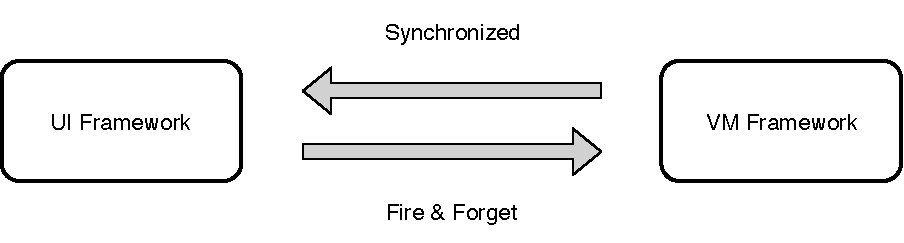
\includegraphics[width=0.8\linewidth]{images/implementation/vmconcurrency.pdf}
	}
	\caption{Synchronization of \ac{VM} and \ac{UI}.}
	\label{fig:vmconcurrency}
\end{figure}

\subsection{Proof of Concept}


\subsection{Core Rules}























